\documentclass[a4paper,11pt]{article}

\usepackage[english]{babel} 
\usepackage[utf8]{inputenc}
\usepackage[cyr]{aeguill}
\usepackage{stmaryrd}

\usepackage{lmodern} %Type1-font for non-english texts and characters
\usepackage{caption}
\usepackage{subcaption}

\usepackage{graphicx}
\usepackage{hyperref}

\usepackage{epstopdf}
\usepackage{multirow}

%% Math Packages 
\usepackage{amsmath}
\usepackage{amsthm}
\usepackage{amsfonts}
\usepackage{amssymb}
\usepackage{mathrsfs}
\usepackage{pst-all}
\usepackage{lscape}
\usepackage{pdfpages}
\usepackage{mathabx}


\usepackage{color, colortbl}
\definecolor{lightgray}{gray}{0.85}
\usepackage{multirow}
\usepackage[Algorithme]{algorithm}
\usepackage[noend]{algpseudocode}
\usepackage{tikz}


\usepackage{a4wide} %%Smaller margins = more text per page.
\usepackage{fancyhdr} %%Fancy headings

\setcounter{secnumdepth}{5}
\setcounter{tocdepth}{5}

\begin{document}

%\pagestyle{fancy}

\begin{center}

\includegraphics[scale=0.4]{GT_logo.jpeg}
\end{center}
\vspace*{\stretch{1}}
\hrulefill
\begin{center}\bfseries\huge
   HW3 Report \\
    Logistic regression\\
    \hrulefill
\end{center}
\vspace*{1cm}
\begin{minipage}[t]{0.4\textwidth}
  \begin{flushleft} \large
    \emph{Subject : \\
    CS 6242 Spring 2017 - OMS}\\
  \end{flushleft}
\end{minipage}
\begin{minipage}[t]{0.6\textwidth}
  \begin{flushright} \large
    \emph{Author :} \\
    Melisande Zonta Roudes \\
    GT account name : mzr3 \\
  \end{flushright}
\end{minipage}
\vspace*{\stretch{2}}
\begin{flushright}
        \today 
\end{flushright} 

\newpage

\section{Data Preprocessing}

The dataset provides 785 rows (784 rows plus one for labels) and 24217 columns for train (4017 for test).
This dataset is inverted indeed usually the attributes stand in the columns and the training examples in the rows. Our data are images so the 784 attributes are pixel (image of $28\times28$). Some operations have to be done to give the appropriate representation of these images. The images are handwritten figures : 0, 1, 3 and 5. It will be the basis of a classification survey between those figures, a binary one.

\begin{figure}[!ht]
\centering
\begin{tabular}{cc}
	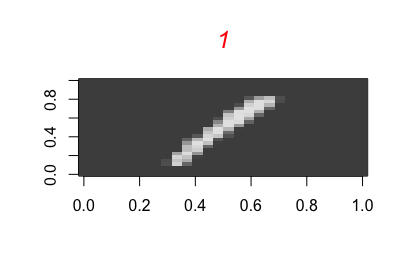
\includegraphics[width=.3\textwidth]{image_1}&
	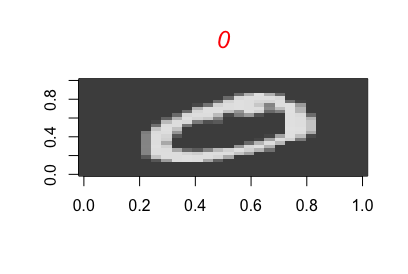
\includegraphics[width=.3\textwidth]{image_0}\\
	a&b\\
	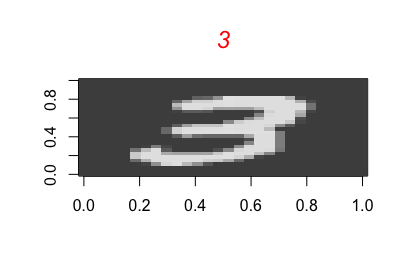
\includegraphics[width=.3\textwidth]{image_3}&
	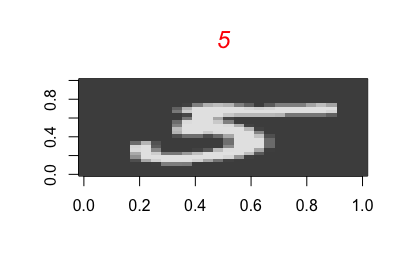
\includegraphics[width=.3\textwidth]{image_5}\\
	c&d\\
\end{tabular}
\caption{\textit{a}. Image digit 1. \textit{b}. Image digit 0. \textit{c}. Image digit 3. \textit{d}. Image digit 5}
\label{images}
\end{figure}

\section{Theory}

\paragraph*{a. Demonstration}

The logistic regression which will be covered here is the one using the batch gradient descent method.

In this part, we will use several notations : 
\begin{itemize}
\item n the number of examples
\item d the dimensionality
\item x the vector of input $\mathbf{x}\in \mathbb{R}^{n\times d}$
\item y the vector of labels which in our case 0/1  $\mathbf{y}\in \mathbb{R}^{n\times1}$
\item $\theta$ vector of weights $\mathbf{\theta}\in \mathbb{R}^{d\times1}$
\end{itemize}

We will consider the logistic function known as sigmoid function $$g(z) = \frac{1}{1 + e^{-z}}$$ The shape of this function shows that it is bounded between 0 and 1. In the hypothesis $h_{\theta}(x)$, we know that  $$h_{\theta}(x) = g(\theta^T x)$$ One of the main interest of the sigmoid function is that it is derivable :
\begin{align*}
g'(z) &= \frac{d}{dz} \frac{1}{1 + e^{-z}}\\
&= \frac{1}{(1 + e^{-z})^2} (e^{-z})\\
&= \frac{1}{1 + e^{-z}} \times (1 - \frac{1}{1 + e^{-z}})\\
&= g(z)(1-g(z))
\end{align*}
In order to perform true logistic regression on our data we put in place the convention of $x_0$ equal to 1 so that $$\theta^{T} x = \theta_{0} + \sum _{j=1}^{n} \theta_j x_j $$
In order to fit our $\theta$ to the logistic regression model, let's write the probabilistic assumptions 

\begin{align*}
P(y = 1 | x;\theta) &= h_{\theta}(x)\\
P(y = 0 | x;\theta) &= 1 - h_{\theta}(x)
\end{align*}
which can be written with a Bernouilli formula as $$p(y | x;\theta) = (h_{\theta}(x))^{y} (1-(h_{\theta}(x)))^{1-y}$$.
In order to determine the maximum likelihood, we determine first the likelihood of the parameters. Indeed as the training examples are independent, we obtain : 

\begin{align*}
L(\theta) &= p(y|X,\theta)\\
&= \prod_{i=1}^n p(y_{i} |X_{i},\theta)\\
&= \prod_{i=1}^n (h_{\theta}(x^{i}))^{y^{i}} (1 - h_{\theta}(x^{i}))^{1 - y_{i}}
\end{align*}

In order to determine the maximum, we transform the previous expression into a logarithmic one.

\begin{align*}
l(\theta) &= \log(L(\theta))\\
&= \sum_{i = 1}^n [y_{i} \log(h_{\theta}(x^{i})) + (1 - y_i) \log(1 - h_{\theta}(x^{i})))]
\end{align*}

By normalizing the function, we obtain the loss function. Since we want to perform gradient descent, we are trying to minimize the negative likelihood.

\begin{align*}
J(\theta) &= -\frac{1}{n}\sum_{i=1}^{n}[ y_{i} \log(h_{\theta}(x^{i})) + (1 - y_i) \log(1 - h_{\theta}(x^{i}))]
\end{align*}

Now we have the expression of the negative log likelihood, we differentiate the expression so we can find the maximum.

\begin{align*}
\frac{\partial J(\theta)}{\partial \theta_{j}} &= -\frac{1}{n}[(y_i \frac{1}{h_{\theta}(x^{i})} - (1-y_i) \frac{1}{1-h_{\theta}(x^{i})})\frac{\partial h_{\theta}(x^{i})}{\partial \theta_{j}}]\\
&= -\frac{1}{n}[(y_i \frac{1}{h_{\theta}(x^{i})} - (1-y_i) \frac{1}{1-h_{\theta}(x^{i})})h_{\theta}(x^{i}) (1- h_{\theta}(x^{i})) \frac{\partial {\theta^T x^{i}}}{\partial \theta_{j}}] \\
&= -\frac{1}{n}[(y_i(1 - h_{\theta}(x^{i})) - (1 - y_i)h_{\theta}(x^{i}))x^{i}_{j}]\\
&= -\frac{1}{n}[(y_i - h_{\theta}(x^{i}))x^{i}_{j}]
\end{align*}

Therefore the $\theta$ update is  : 
$$ \theta = \theta - \alpha \nabla_{\theta} J(\theta) $$ with the gradient of the loss function written as :  $$\nabla_{\theta} J(\theta) = -\frac{1}{n}[(y - h(\theta^{T}x))x^{T}]$$ 

\paragraph*{b. Pseudo Code}

The implementation of the logistic regression includes several steps like the calculation of the cost function which is the derivative of the loss function and then the update of our weights vector.

\begin{algorithm}[H]
\caption{Training a model using Logistic Regression.}
\begin{algorithmic}[1]
\State Binarize the labels of the dataset (conversion to 0/1)
\State Add a column of ones to X which represents the constant X = [ones(n,1) X]
\State Initialisation  of the weights vector $\mathbf{\theta} = [0, 0, ..., 0]^{T}$
\State h(x) = $\frac{1}{1 + e^{-x}}$
\While{convergence-criterion > threshold}
\State $\theta$ = $\theta$ - $\alpha$ $\times$ $\nabla_{\theta}J(\theta)$
\State $\alpha$ = $\alpha$ $\times$ 0.9
\EndWhile
\end{algorithmic}
\end{algorithm}

As described in the videos, a decreasing learning rate was chosen in order to accelerate the convergence and avoid a possible overfitting.\\
The stopping criteria of this algorithm are various but two of them caught my attention. 
\begin{itemize}
	\item[-] The most natural one seems to be to compute the norm 2 (euclidean norm) of the difference between two successive vector $\theta$. In this way, we come up with the computation of the euclidean norm of the multiplication of the learning rate and the cost function. We stop when a threshold is reached on this criteria or when the maximum of iterations is reached (in the case of a non convergence).
	\item[-] The second one is linked to the first one since we will consider the difference of values of the logistic loss over the successive iterations. Indeed, it's interesting to consider the loss function which is the primitive of the cost function which gives different informations than the cost function multiplied by $\alpha$.
\end{itemize}

\paragraph*{c. Other details}

With d the dimensionality of $\theta$ and n the number of training examples, we consider the gradient descent function which calls cost-function and sigmoid functions : 4 operations are computed in the sigmoid function, $(y - h(\theta^{T}x)$ in the gradient is computed in n(8d-3) operations since the sigmoid function is applied to the 2d-1 operations for $\theta^T X_i$ (so 8d-4) plus we do 1 operation for the substraction and finally it is done for each training example, $(y - h(\theta^{T}x))X^{T}$ is adding d(2n-1 )operations, then the normalization by n adds 3d operations and finally the decrease of the learning rate adds 2d operations.
Hence the complexity is $O(n\times d)$.

\section{Implementation}

In order to implement the pseudo code below, three functions were created : 
\begin{enumerate}
\item  Sigmoid function
\item  Cost Function
\item  Gradient descent with the two types of convergence criteria mentioned above
\end{enumerate}

\section{Training}

\paragraph*{a.} 
The convergence criterion chosen is the first one (euclidean norm of the difference of $\theta$) and the threshold is set to $10^{-3}$ and the maximum iterations is 3000.
In order to evaluate the algorithm we have implemented before, a function accuracy was created. It's role is to compare the output created from the weights vector $\theta$ and to compare it with the dataset's labels.

\begin{table}[H]
\centering
\caption{Training and testing accuracies over one iteration}
\label{one iteration}
\begin{tabular}{c|c|c|c|}
\cline{2-4}
                                         & Training Accuracy & Test Accuracy & Number of iterations \\ \hline
\multicolumn{1}{|c|}{Classification 0/1} & 99.65259 $\%$       & 99.85816 $\%$   & 30                   \\ \hline
\multicolumn{1}{|c|}{Classification 3/5} & 92.62465 $\%$      & 94.00631 $\%$   & 41                   \\ \hline
\end{tabular}
\end{table}

As we can see in the table \ref{one iteration}, the accuracies are really high for the dataset 0/1 with an higher value for the testing than the training. The classification 3/5 is not performed as well as 0/1, but the increase in the testing rate is much more visible. We can also see the difficulty to converge since the number of iterations is higher in the classification 3/5 than in the 0/1.

\paragraph*{b.} 

As highlighted in the notes of this question, I encountered the classical problem of the batch method which is that over 10 iterations, we will obtain the same accuracy. To solve this problem, we randomly shuffle the data by sampling on $80\%$. 

\begin{figure}[!ht]
\centering
\begin{tabular}{cc}
	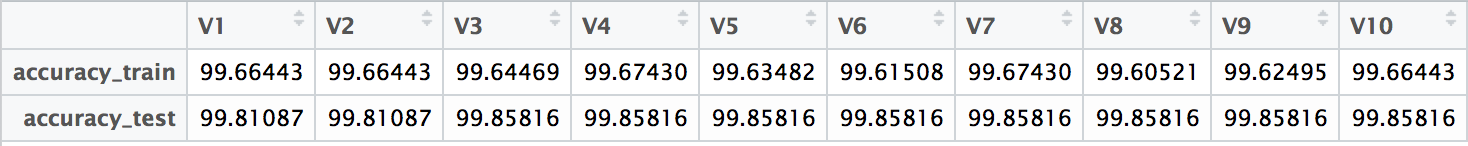
\includegraphics[width=.9\textwidth]{10_iterations_0_1}\\
	a.\\
	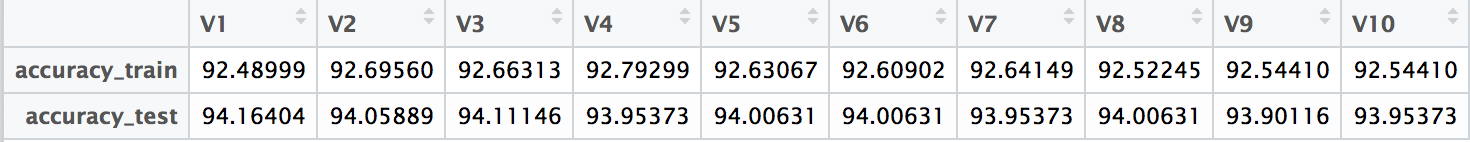
\includegraphics[width=.9\textwidth]{10_iterations_3_5}\\
	b.\\
\end{tabular}
\caption{\textit{a}. Classification between 0 and 1 over 10 iterations. \textit{b}. Classification between 3 and 5 over 10 iterations. }
\label{tables}
\end{figure}

We can visualize on the figures $\ref{tables}$ that the accuracies are different so the technique is working, we don't obtain a value repeated 10 times.s

\begin{table}[H]
\centering
\caption{Training and testing accuracies over 10 iterations}
\label{10 iterations}
\begin{tabular}{c|c|c|}
\cline{2-3}
 & Training Accuracy & Test Accuracy \\ \hline
\multicolumn{1}{|c|}{Classification 0/1} & 99.64666 $\%$ & 99.8487 $\%$ \\ \hline
\multicolumn{1}{|c|}{Classification 3/5} & 92.61335 $\%$ & 94.01157 $\%$ \\ \hline
\end{tabular}
\end{table}

The results are really close as we can see but as their represent an average over multiple iterations, they are more trusted values than random results that occur on one iteration.

\paragraph*{c.}

The difference between the classification of 0/1 and 3/5 is directly linked to the shape of our figures we have seen in the first part. Indeed, the figures 0 and 1 have nothing in common, so the number of pixels in common is really small whereas the curve present in the low part of 3 and 5 are absolutely similar, which makes of those figures half similar. From those observations, we can understand the difference of results in accuracy and the difficulty to converge towards our threshold.


\paragraph*{d.}

Although this logistic regression task was designed for binary classification, several classes can be handled also by this method. A common strategy is to use multiple binary classifiers to decide on a single-best class for new instances. We may create a classifier for each class in a one-versus-all way then, for new points, classify them based on the classifier function that produces the largest value. An other method could be to set up classifiers comparisons and select class that 'wins' the most pairwise matchups for new points. 

\section{Evaluation}

In order to perform well on our classification, some parameters can be tuned as the initialization vector and all about the stopping criteria (maximum of iterations, threshold or convergence criteria). In this section, we will do some tests on the parameters but the maximum of iterations and threshold remain the same ( max.iterations = 3000 and conv.criterion = $10^{-3}$) in order to make some suitable comparisons with our previous results.

\paragraph*{a.} 

The initial weight vector was a vector of zeros. As the input values are bound between 0 and 1, we will determine if it's easier to converge if $\theta = [0, 0, ..., 0]^{T}$ or with a $\theta$ composed randomly of 0's and 1's.

\begin{table}[H]
\centering
\caption{Change in the initialization of the weight vectors}
\label{change_init}
\begin{tabular}{c|c|c|l}
\cline{2-4}
 & Training Accuracy & Test Accuracy & \multicolumn{1}{l|}{Number of Iterations} \\ \hline
\multicolumn{1}{|c|}{1 iteration} & 83.85561 \% & 85.75184 \% & \multicolumn{1}{c|}{51} \\ \hline
\multicolumn{1}{|c|}{10 iterations} & 85.19965 & 86.49317 &  \\ \cline{1-3}
\end{tabular}
\end{table}

As a recall, the number of iterations for 3/5 classification was 41 and the accuracy was around 92-94 $\%$ so this initialization vector represents a huge obstacle to converge and the accuracy obtained (around $83-86 \%$) is worse than with the baseline criterion.

\paragraph*{b.}

As detailed in the pseudocode, the first convergence criterion was based on the cost function whereas the second is on the loss function. It evaluates different behaviours.

\begin{table}[H]
\centering
\caption{Change in the convergence criteria}
\label{change_converg}
\begin{tabular}{c|c|c|l}
\cline{2-4}
 & Training Accuracy & Test Accuracy & \multicolumn{1}{l|}{Number of Iterations} \\ \hline
\multicolumn{1}{|c|}{1 iteration} & 92.19183 \% & 93.74343 \% & \multicolumn{1}{c|}{17} \\ \hline
\multicolumn{1}{|c|}{10 iterations} & 92.253 \% & 93.75394 \% &  \\ \cline{1-3}
\end{tabular}
\end{table}

As we can see on the table \ref{change_converg}, the accuracies are rather the same than the baseline results. There is a slight difference indeed the second criterion provide less good results that the first one but the number of iterations is remarkably lower (17 on the second instead of 41 for the first one).

\section{Learning Curves}

In conclusion of these tests, the best way to experiment the behaviour of our logistic regression algorithm on our dataset is to draw learning curves (training curves and testing ones). In this part, we will test our accuracy and logistic loss on different splits of our dataset. The splits were done 5 by 5 from $5\%$ to $100\%$.

\paragraph*{a. Accuracy curves}

\begin{figure}[H]
\centering
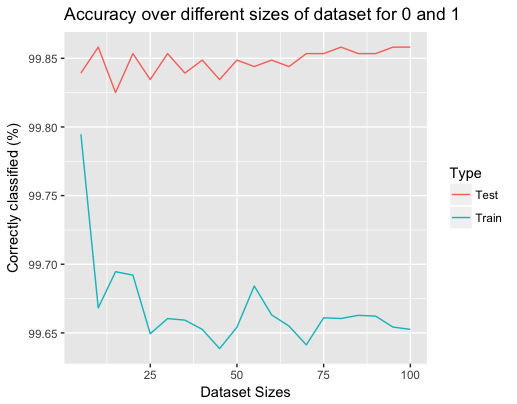
\includegraphics[width=.6\textwidth]{0_1_accuracy}
\caption{Learning curve for the classification between 0's and 1's}
\label{0_1_accuracy}
\end{figure}

The training curves and testing curves on figure \ref{0_1_accuracy} do not provide much information since we can see that the test accuracy is constant (around $99.85\%$ for the testing accuracy and  between $99.65\%$ and $99.80\%$ for the training) over the different dataset sizes and although the train set seems to have a different variation, the peaks are not relevant. By looking at the range of values, we can see that the minimal and maxima are really close. The second striking observation is the fact that the test accuracy is much higher than the train one which is unusual. This could be explained by the fact that in our code we randomly shuffle split our train data in order to obtain our $\theta$ from the gradient descent method whereas we keep the test dataset the same, no shuffle split is done. So from these observations we could say that the test set is easier for the classification between 0 and 1 in comparison to the shuffled split training dataset.

\begin{figure}[H]
\centering
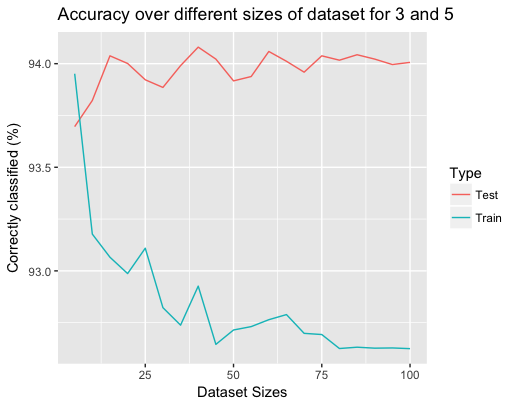
\includegraphics[width=.6\textwidth]{3_5_accuracy}
\caption{Learning curve for the classification between 3's and 5's}
\label{3_5_accuracy}
\end{figure}

The training and testing curves on figure \ref{3_5_accuracy} for the 3/5 classification are a lot more interesting. Just by observing the range we can see that this one is more relevant (around $1.5\%$ of variation) than the 0/1 classification indeed for the testing the accuracy goes from $93.54\%$ to $94.0\%$ and for the training it went down from $94.0\%$ to almost $92.5\%$. We notice a decreasing behaviour of the train set and a slightly increasing variation of the test set. This can be explained by the fact that the more data the learner has to train one the less the accuracy is good. Indeed, training on 1210 examples is easier than training on 24217 examples. The test accuracy has a logical behaviour since the more the learner trains, the better the test is successful. The inversion of train and test curves has the same explanation mentioned above.

\paragraph*{b. Logistic loss curves}

As the accuracies were meaningful, the logistic loss is another representative parameter. Indeed loss functions represent the price paid for inaccuracy of predictions in classification problems. 

\begin{figure}[H]
\centering
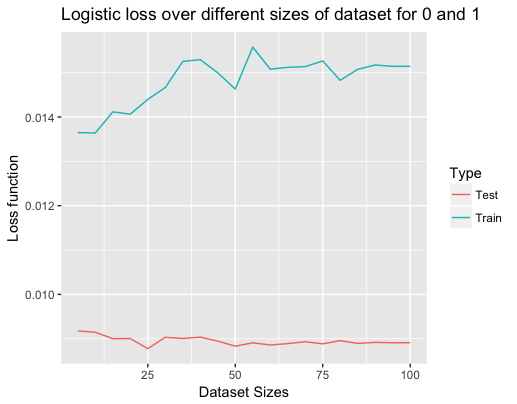
\includegraphics[width=.6\textwidth]{0_1_loss}
\caption{Logistic loss curve for the classification between 0's and 1's}
\label{0_1_loss}
\end{figure}

The constancy of the training and testing curves on figure \ref{0_1_loss} (for the testing around 0.009 and between 0.014 and 0.015) has been mentioned in the first part on the accuracy training and testing curves. The difference between the previous curves and these ones stand in the inversion between the training set curve and the testing set curve, which is logical since the loss function represents somehow the inaccuracy. 

\begin{figure}[H]
\centering
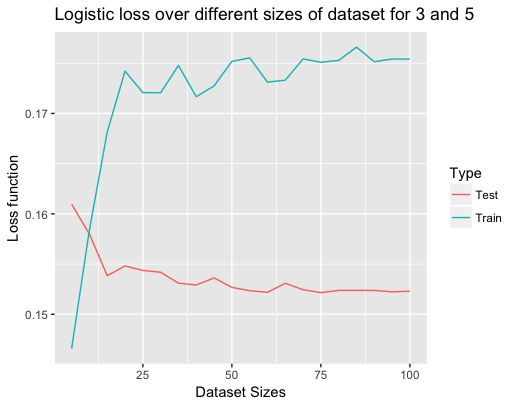
\includegraphics[width=.6\textwidth]{3_5_loss}
\caption{Logistic loss curve for the classification between 3's and 5's}
\label{3_5_loss}
\end{figure}

The inversion of the training curves and testing curves can also be seen on figure \ref{3_5_loss}, and we can observe as well the increasing behaviour of the train set and the decreasing one for test set. The testing accuracy goes from 0.16 to 0.152 and the training accuracy from 0.148 to 0.175.

\end{document}
